\input{../YKY-preamble.tex}
\setmainfont[BoldFont=Alibaba_Sans_Regular.otf,ItalicFont=Alibaba_Sans_Light_Italic.otf]{Alibaba_Sans_Light.otf}

% \usepackage[backend=biber]{biblatex}
% \bibliography{../AGI-book}

\usepackage[active,tightpage]{preview}		% for continuous page(s)
\renewcommand{\PreviewBorder}{0.5cm}
\renewcommand{\thempfootnote}{\arabic{mpfootnote}}

\usepackage[absolute,overlay]{textpos}		% for page number on upper left corner

\usepackage{color}
\usepackage{mathtools}
\usepackage[hyperfootnotes=false]{hyperref}

% \usepackage[backend=biber,style=numeric]{biblatex}
% \bibliography{../AGI-book}
% \renewcommand*{\bibfont}{\footnotesize}

\usetikzlibrary{shapes}
\usepackage[export]{adjustbox}				% ??
\usepackage{verbatim} % for comments
% \usepackage{newtxtext,newtxmath}	% Times New Roman font

% \titleformat{\subsection}[hang]{\bfseries\large\color{blue}}{}{0pt}{} 
% \numberwithin{equation}{subsection}

\newcommand{\underdash}[1]{%
	\tikz[baseline=(toUnderline.base)]{
		\node[inner sep=1pt,outer sep=10pt] (toUnderline) {#1};
		\draw[dashed] ([yshift=-0pt]toUnderline.south west) -- ([yshift=-0pt]toUnderline.south east);
	}%
}%

\newcommand\reduline{\bgroup\markoverwith{\textcolor{red}{\rule[-0.5ex]{2pt}{0.4pt}}}\ULon}

%\DeclareSymbolFont{symbolsC}{U}{txsyc}{m}{n}
%\DeclareMathSymbol{\strictif}{\mathrel}{symbolsC}{74}
\DeclareSymbolFont{AMSb}{U}{msb}{m}{n}
\DeclareSymbolFontAlphabet{\mathbb}{AMSb}
% \setmathfont{Latin Modern Math}
\DeclareMathOperator*{\argmin}{arg\,min}

% \usepackage[most]{tcolorbox}
\tcbset{on line, 
	boxsep=4pt, left=0pt,right=0pt,top=0pt,bottom=0pt,
	colframe=red,colback=pink,
	highlight math style={enhanced}
}
\newcommand{\atom}{\vcenter{\hbox{\tcbox{....}}}}

\let\oldtextbf\textbf
\renewcommand{\textbf}[1]{\textcolor{blue}{\oldtextbf{#1}}}

\newcommand{\logic}[1]{{\color{violet}{\textit{#1}}}}
\newcommand{\underconst}{\includegraphics[scale=0.5]{../2020/UnderConst.png}}
\newcommand{\KBsymbol}{\vcenter{\hbox{\includegraphics[scale=1]{../KB-symbol.png}}}}
\newcommand{\token}{\vcenter{\hbox{\includegraphics[scale=1]{token.png}}}}
\newcommand{\proposition}{\vcenter{\hbox{\includegraphics[scale=0.8]{proposition.png}}}}

\newcommand{\circled}[1]{{\textcircled{\sffamily \scriptsize{#1}}}}

\begin{document}

\begin{preview}

\cc{
\title{\vspace{-1.5cm} \bfseries\color{blue}{\LARGE Further Interpreting the Transformer}}
}{
\title{\vspace{-1.5cm} \bfseries\color{blue}{\LARGE Further Interpreting the Transformer}}
}

% \author{YKY} % Your name
\date{\vspace{-2cm}} % Date, can be changed to a custom date

\maketitle

\setcounter{section}{-1}

% (1) Circled page number on upper left corner
% \begin{textblock*}{5cm}(2.1cm,2.3cm) % {block width} (coords) 
% {\color{red}{\large \textcircled{\small 1}}}
% \end{textblock*}

\begin{minipage}{\textwidth}
\setlength{\parskip}{0.4\baselineskip}

This is an illustration of how the Transformer processes tokens:
\begin{equation}
\vcenter{\hbox{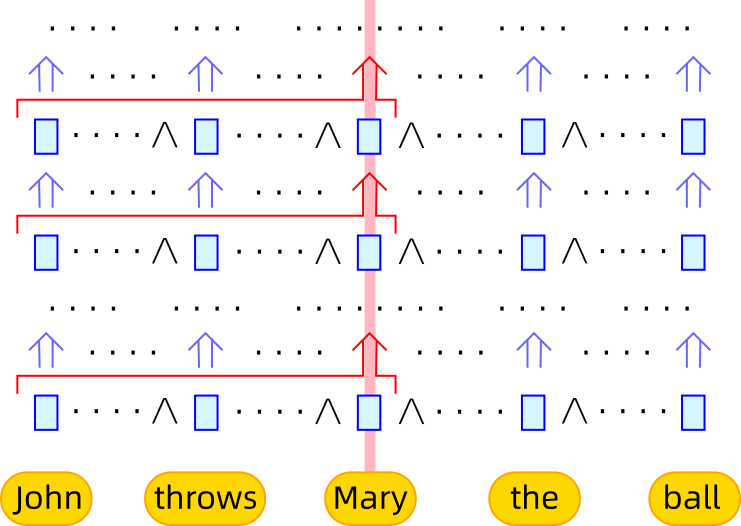
\includegraphics[scale=1]{Transformer-pivot-and-axis.png}}}
\end{equation}

\begin{itemize}
\item The Transformer is basically a neural network function or mapping that accepts a \textbf{sequence} token by token, and outputs a new token per each input token.  The output of each token is equivalent to looking up a \textbf{logic rule base} with premises drawn from the input tokens.
	
\item \cc{
	Transformer 的一次 变换 是以某个 token 作为 支点 (pivot) 或 主轴(红色粗线)再结合其他 tokens 的 叠加讯息。}{
	Each pass of Self-Attention has an \textbf{axis} (thick red line), where a \textbf{pivot} token is combined with other tokens via super-position. \\
	Why do pivots exist?  The pivot is the \textbf{latest} token being added to the ``state'' of the system, ie, the sequence of tokens up to time $t$.  The rest of the state has not changed except for this ``delta'' token.  Therefore, the logical conclusions that were drawn up to time $t-1$ has already been outputted.  What we need to do is to output the new conclusions that is now deducible from the newest token and the rest of the state.  This situation is completely analogous to ``rule-based systems'' in the old days, eg. the SOAR architecture, where tokens are called WMEs (working memory elements).
}

\item \cc{
	每个 token 似乎是时间 0....t 的句子 前缀 的内容概括。这内容概括似乎是分布式的表示,但也可能有 softmax 的选择性的解偶 (disentanglement).}{
	Each token seems to be the ``summary'' of the incoming tokens up to time $t$.  Such a summary seems to be a distributive representation made of superpositions of values $V = W^V X$, but due to the action of \textit{softmax}, some tokens may be \textbf{selected} over others.  This may have the effect of \textbf{disentangled representations} that are closer to symbolic logic.
}

\item We want to see if Self-Attention can perform ``variable substitution'' in  logic rules.  This requires extracting some vector components of a token and copying them to the next layer.  But this operation varies from rule to rule.  
\end{itemize}

\end{minipage}
\end{preview}
\end{document}
